\documentclass[12pt]{IEEEtran}
\usepackage[utf8]{inputenc}
\usepackage{graphicx}
\usepackage{amsmath, amsthm, amssymb}

\title{Chaos Project 1}
\author{
  Paul Booth \\
  \and
  Geoff Pleiss
}
\date{}

\newtheorem{thm}{Theorem} 
\newtheorem{lma}{Lemma}

\begin{document}
  \maketitle 

\begin{abstract}
\end{abstract}



\section{Introduction}
The theorem we are trying to prove is

\begin{thm}
\label{thm:mainthm}
	Let $J$ be an interval and let $F$ be a continuous first-order map with $F : J \rightarrow J$. If there is some point $a \in J$ that satisfies the following
	%
	\[ F^3\left(a\right) \leq a < F\left(a\right) < F^2\left(a\right) \]
	or
	\[ F^3\left(a\right) \geq a > F\left(a\right) > F^2\left(a\right) \]
	%
	then $J$ contains a $k$-period orbit for all $k \in \mathbb{N}$.
\end{thm}

In the first section we will provide a rough outline of the proof for this theorem, which will be followed by the proof in full. We will then discuss the interpretations and implications of our results.

\section{The big picture}




\section{Lemmas}
% TODO: FIGURE OUT HOW WE WANT TO PRESENT THIS ACTUALLY

\begin{lma}
\label{lma:cont_comp}
	Continuity / compactness
\end{lma}

\begin{figure}
\label{fig:continuity_graph}
	\begin{center}
		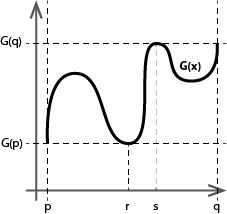
\includegraphics{img/continuity_graph.png}
		\caption{Diagram for Lemma \ref{lma:cont_comp}}
	\end{center}
\end{figure}


\section{Implications/Conclusions}




\end{document}

